\documentclass{beamer}
\title{What is Read-Copy Update?}
\subtitle{RCU in HelenOS}
\usetheme{CambridgeUS}
\usecolortheme{beaver}
\usepackage{algorithmic}
\usepackage{graphics}
\usepackage{listings}
\usepackage{booktabs}
\usepackage{local_dir}
\graphicspath{ {\rcufigure/helenOS/}}
\lstset{inputpath=\rcucode/helenOS/,
  basicstyle=\scriptsize,
  numbers=left,
  xleftmargin=10pt,
  tabsize=2,
}
\author{Chang-Hui Kim}

\begin{document}

\begin{frame}
  \titlepage
\end{frame}

%% -------------------------------------------------------------------------

\begin{frame}[t]
  \frametitle{What is Read-Copy Update?}

  \begin{itemize}
  \item designed to enable scalable concurrent read access to data that is mostly read.
    (Write ratio 10\%$\sim$40\%)
  \item allows readers to execute concurrently \textbf{with updaters}.
  \item While an update is in progress RCU
    \begin{itemize}
    \item maintains older versions of the data.
    \item ensures readers always access coherent albeit possibly outdated data.
    \end{itemize}
  \item efficiently propagate new versions of objects.
  \item defer reclamation of old objects until they are no longer referenced.
  \end{itemize}
  
\end{frame}

%% -------------------------------------------------------------------------

\section{Semantics}

%% -------------------------------------------------------------------------

\begin{frame}[t]
  \frametitle{RCU readers}

  \begin{itemize}
  \item reference RCU protected data within a \emph{read-side critical section}
    (reader section).
  \item reader sections are delimited by \texttt{Rcu-Read-Lock} and
    \texttt{Rcu-Read-Unlock}.
  \item these functions never block.
  \end{itemize}

  \begin{figure}[ht]
    \centering
    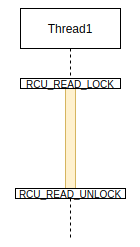
\includegraphics[width=0.2\textwidth]{reader_thread_ex.png}
  \end{figure}

  
\end{frame}

%% -------------------------------------------------------------------------

\begin{frame}[t]
  \frametitle{RCU terminology}

  \begin{itemize}
  \item If a thread is not executing a read-side critical section it is said to be
    in a \emph{quiescent state}.
  \item Any time period such that each \textbf{thread passes through at least
    one quiescent state} is called a \emph{grace period}.
  \end{itemize}
  
  \begin{figure}[ht]
    \centering
    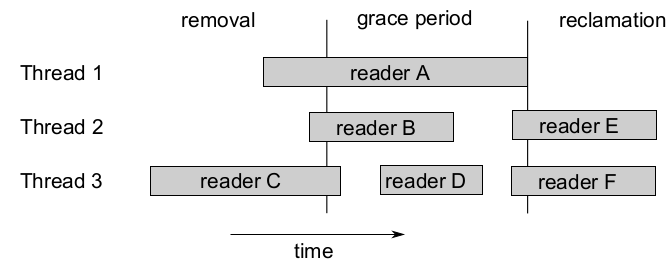
\includegraphics[width=0.7\textwidth]{grace_period.png}
    \caption{sequence of linked-list removal}
  \end{figure}

\end{frame}

%% -------------------------------------------------------------------------

\begin{frame}[t]
  \frametitle{RCU terminology}

  \begin{figure}[ht]
    \centering
    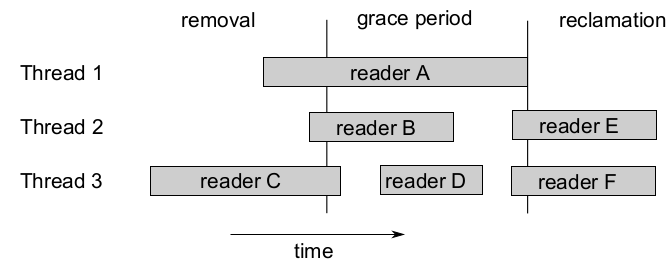
\includegraphics[width=0.7\textwidth]{grace_period.png}
    \caption{sequence of linked-list removal}
  \end{figure}

  \begin{itemize}
  \item any critical sections \textbf{existing at the beginning of a grace period}
    will have completed before the grace period ends. (A, B, C)
  \item threads continuously entering RCU critical sections don't prolong a grace period.
    (D, E, F)
  \end{itemize}
  
\end{frame}

%% -------------------------------------------------------------------------

\begin{frame}[t]
  \frametitle{RCU updaters}
  
  \begin{itemize}
  \item Updaters use grace periods to effect deffered destruction.
  \item All readers that may have been using the element must have completed
    by the time \texttt{Rcu-Synchronize} returns.
  \end{itemize}

\end{frame}

%% -------------------------------------------------------------------------

\begin{frame}[t]
  \frametitle{RCU removal example}
  
  In particular, to remove an element from a data structure,
  \begin{enumerate}
  \item unlinks the element from the data structure.
  \item invokes \texttt{Rcu-Synchronize}, which waits for a grace period to elapse.
  \item it is safe to reclaim or free the unlinked element.
  \end{enumerate}

  \begin{figure}[ht]
    \centering
    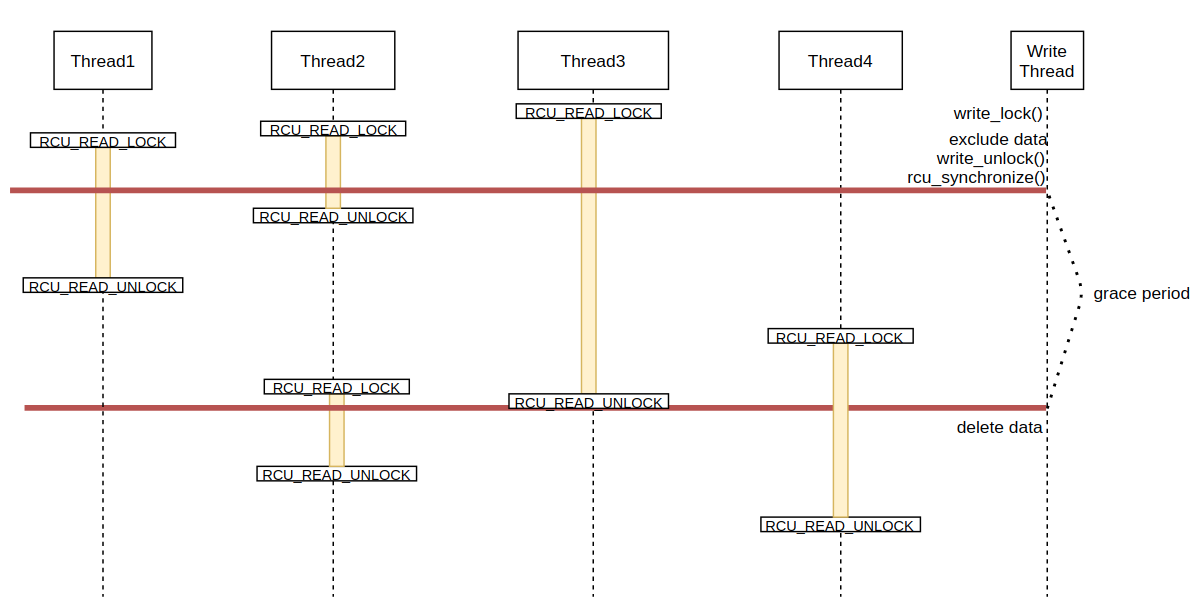
\includegraphics[width=1\textwidth]{rcu_sequence.png}
  \end{figure}
  
\end{frame}

%% -------------------------------------------------------------------------

\begin{frame}[t]
  \frametitle{RCU removal example}

  \begin{figure}[ht]
    \centering
    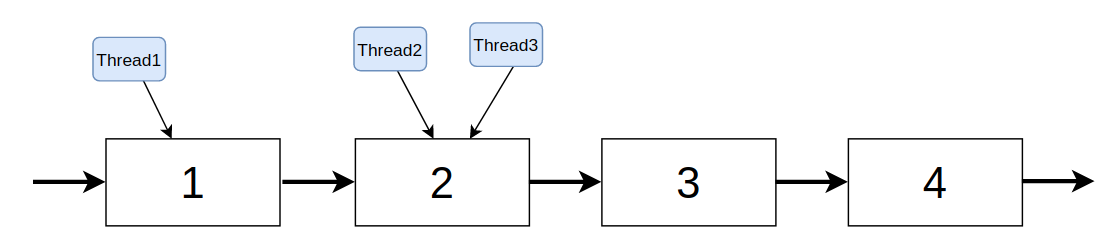
\includegraphics[width=1\textwidth]{rcu_del_1.png}
    \caption{initial state}
  \end{figure}
  
\end{frame}

%% -------------------------------------------------------------------------

\begin{frame}[t]
  \frametitle{RCU removal example}

  \begin{figure}[ht]
    \centering
    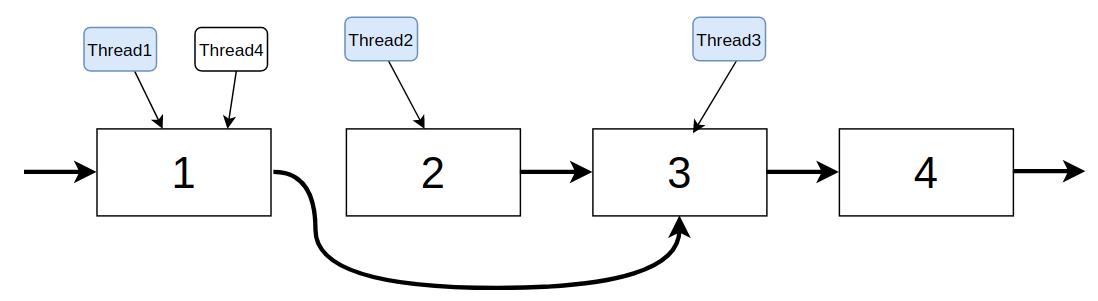
\includegraphics[width=1\textwidth]{rcu_del_2.png}
  \end{figure}

  \begin{enumerate}
  \item unlinks the element from the data structure.
  \item invokes \texttt{Rcu-Synchronize}, which waits for a grace period to elapse.
  \end{enumerate}
  
\end{frame}

%% -------------------------------------------------------------------------

\begin{frame}[t]
  \frametitle{RCU removal example}

  \begin{figure}[ht]
    \centering
    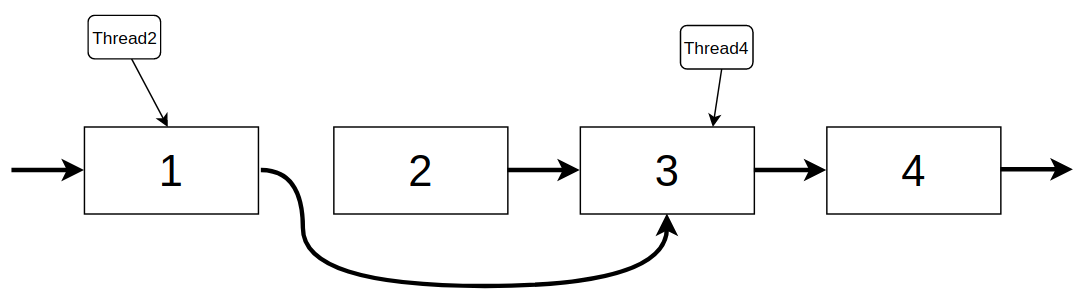
\includegraphics[width=1\textwidth]{rcu_del_3.png}
    \caption{after \texttt{Rcu-Synchronize} returned.}
  \end{figure}
  
\end{frame}

%% -------------------------------------------------------------------------

\begin{frame}[t]
  \frametitle{RCU removal example}

  \begin{figure}[ht]
    \centering
    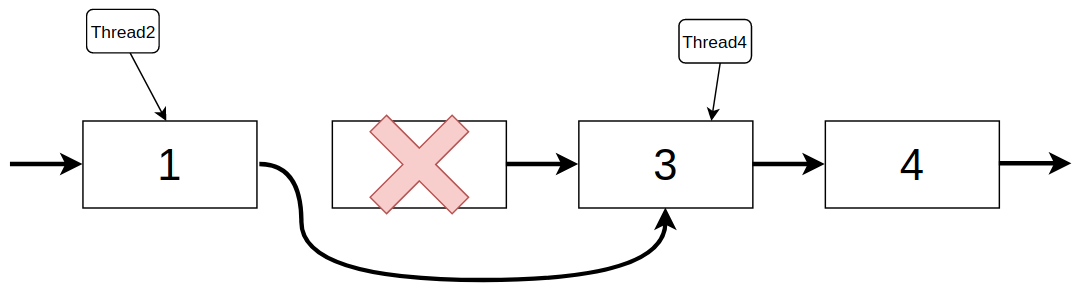
\includegraphics[width=1\textwidth]{rcu_del_4.png}
    \caption{it is safe to reclaim or free the unlinked element.}
  \end{figure}
  
\end{frame}

%% -------------------------------------------------------------------------

\begin{frame}[t]
  \frametitle{note}

  \begin{itemize}
  \item RCU only coordinates the concurrent execution of a reader with other readers or
    updaters.
  \item However, it in no way synchronizes updaters with other updaters. (So use lock)
  \end{itemize}
  
\end{frame}

%% -------------------------------------------------------------------------

\section{Example usage}

%% -------------------------------------------------------------------------

\begin{frame}[t]
  \frametitle{Example usage}

  RCU example of working with a single linked null terminated list.
  
  \lstinputlisting[firstline=1, lastline=9]{example_usage.c}

  \begin{itemize}
  \item \texttt{first} can be read in parallel as it is protected by RCU.
  \item RCU protects only the list’s links \texttt{next}.
  \item assumes \texttt{value}, does not change after an element is inserted.
  \item The list is protected from concurrent modifications with a single mutex
    \texttt{update\_mtx}.
  \end{itemize}

\end{frame}

%% -------------------------------------------------------------------------

\begin{frame}[t]
  \frametitle{Read Side}

  \lstinputlisting[firstline=11, lastline=24]{example_usage.c}

  \begin{itemize}
  \item Before accessing any RCU protected fields, enter a reader section. (3)
  \item read the protected field via \texttt{rcu\_access()}.
  \item notify updaters that it is safe to reclaim elements used in
    the reader section. (\texttt{rcu\_read\_unlock()})
  \end{itemize}
  
\end{frame}

%% -------------------------------------------------------------------------

\begin{frame}[t]
  \frametitle{Write Side}

  \lstinputlisting[firstline=26, lastline=34]{example_usage.c}

  \begin{itemize}
  \item The list is changed with the mutex \texttt{list->update\_mtx} locked only.
  \item updaters always have a consistent view of the list.
  \item The new element is published for readers to see by means of \texttt{rcu\_assign()}.
  \end{itemize}
  
\end{frame}

%% -------------------------------------------------------------------------

\begin{frame}[t]
  \frametitle{Write Side}

  \lstinputlisting[firstline=36, lastline=49]{example_usage.c}

  \begin{itemize}
  \item not necessary to \texttt{rcu\_assign()} the address of the second element to
    \texttt{list->first}.
  \item \texttt{rcu\_synchronize()} waits for any readers that may have been accessing the
    removed element to complete.
  \end{itemize}

\end{frame}

%% -------------------------------------------------------------------------

\begin{frame}[t]
  \frametitle{Write Side}
  \begin{figure}[ht]
    \centering
    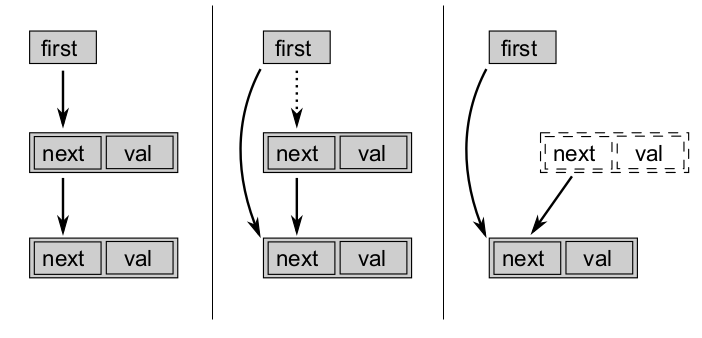
\includegraphics[width=0.8\textwidth]{example_delete.png}
  \end{figure}

\end{frame}

%% -------------------------------------------------------------------------

\section{Complete interface}

%% -------------------------------------------------------------------------

\begin{frame}[t]
  \frametitle{Complete interface}

  \begin{itemize}
  \item \texttt{Rcu-Read-Lock} delimits the start of a read-side critical section.
  \item \texttt{Rcu-Read-Unlock} marks the end of a read-side critical section.
  \item \texttt{Rcu-Synchronize} blocks for an entire grace period.
    \begin{itemize}
    \item waits for any preexisting readers (may accessing old versions of data) to
      complete. 
    \item it guarantees any new readers see changes introduced prior to calling
      \texttt{Rcu-Synchronize} in the same thread.
    \end{itemize}
  \item \texttt{Rcu-Call}
    \begin{enumerate}
    \item returns immediately.
    \item asynchronously invokes a callback function when a grace period elapses.
    \end{enumerate}
  \end{itemize}

\end{frame}

%% -------------------------------------------------------------------------

\begin{frame}[t]
  \frametitle{Complete interface}

  \begin{itemize}
  \item \texttt{Rcu-Barrier} waits for all callbacks queued via \texttt{Rcu-Call} at the
    time of the
    call to \texttt{Rcu-Barrier} to complete.
  \item \texttt{Rcu-Dereference, Rcu-Access} 
    \begin{itemize}
    \item is used to load a pointer to an RCU protected object within a reader section.
    \item prohibits the compiler to reload the pointer as part of optimizations.
    \end{itemize}
  \item \texttt{Rcu-Assign} 
    \begin{itemize}
    \item assigns the address of a new initialized element to an RCU protected pointer.
    \item On weakly ordered architectures, it ensures that initialization of the element
      is visible.
    \end{itemize}
  \end{itemize}
  
\end{frame}

%% -------------------------------------------------------------------------

\section{Constraints on implementations}

%% -------------------------------------------------------------------------

\begin{frame}[t]
  \frametitle{Constraints on implementations}
  The primary sources of the slowdown of traditional locking mechanism.

  \begin{itemize}
  \item Cache misses due to lock variables. (rcu improve this)
  \item Atomic operations. (rcu improve this)
  \item Memory barriers delimiting critical section code lead to pipeline stalls.
  \end{itemize}

\end{frame}

%% -------------------------------------------------------------------------

\begin{frame}[t]
  \frametitle{Memory Barrier}
  Architectures without sequentially consistent memory models are allowed
  to \textbf{aggressively reorder memory accesses}.

  \begin{figure}
    \begin{tabular}{c c}
      CPU1 & CPU2 \\
      \midrule
      X = 1; & Y = 1;\\
      r1 = Y; & r2 = X;
    \end{tabular}
  \end{figure}

  Weakly ordered architectures
  \begin{itemize}
  \item may issue the loads of \emph{X} and \emph{Y} before writing the variables.
  \item provide \textbf{memory barrier} instructions that limit how memory operations
    may be reordered.
  \end{itemize}
  
\end{frame}

%% -------------------------------------------------------------------------

\begin{frame}[t]
  \frametitle{Memory Barrier}
  \textbf{Locks} surround critical section code
  \begin{itemize}
  \item with memory barriers that prevent
    the CPU from issuing loads and stores of protected shared variables \textbf{outside
      the protected region}.
  \item without the barriers CPUs would
    \begin{itemize}
    \item be free to load a shared variable before a mutex is acquired.
    \item write to a shared variable after a mutex is released.
    \end{itemize}
  \end{itemize}
  
\end{frame}

%% -------------------------------------------------------------------------

\begin{frame}[t]
  \frametitle{Memory Barrier}
  RCU algorithms are faced with the same problem.\\

  Without memory barriers in these functions,
  \begin{itemize}
  \item the CPU may be referencing RCU protected data even outside of the read-side critical
    section.
  \item RCU cannot declare that a thread is in a quiescent state just because it is not
    executing instructions within \texttt{Rcu-Read-Lock} and \texttt{Rcu-Read-Unlock}.
  \end{itemize}

\end{frame}

%% -------------------------------------------------------------------------

\begin{frame}[t]
  \frametitle{Memory Barrier}
  RCU may
  \begin{itemize}
  \item issue memory barriers in threads on demand during grace period detection.
  \item wait for naturally occurring memory barriers. (ex, context switch)
  \end{itemize}
  
\end{frame}

%% -------------------------------------------------------------------------

\begin{frame}[t]
  \frametitle{Reference}

  \begin{center}
    \url{http://www.helenos.org/doc/theses/ah-thesis.pdf}
  \end{center}
 
\end{frame}

\end{document}
